The Canada-France-Hawaii Telescope Lensing Survey (CFHTLenS) represented a major step forward for the field of weak gravitational lensing, in terms of improved accuracy in data reduction \citep{erben/etal:2013}, the implementation of PSF-Gaussianised matched multi-band photometry \citep{hildebrandt/etal:2012}, cross-correlation clustering analysis between photometric redshift slices to verify tomographic redshift distributions \citep{benjamin/etal:2013}, accurate calibrated shape measurements \citep{miller/etal:2013} and a full suite of informative systematic tests to select a clean data set \citep{heymans/etal:2012}.    Since the public release of this survey in 2013, the community has continued to scrutinise and advance our understanding of CFHTLenS by identifying a number of areas where analyses could improve:
\begin{itemize}
\item{\citet{choi/etal:2016} identified biases in the tomographic photometric redshift distributions using a more effective clustering analysis, in comparison to \citet{benjamin/etal:2013}, by incorporating newly overlapping spectroscopy from the Sloan Digital Sky Survey.  The CFHTLenS tomographic cosmological analysis was then revisited by \citet{joudaki/etal:2016} in order to include a full redshift error analysis based on the results from \citet{choi/etal:2016}, discussed further in section~\ref{sec:photoz}.}
\item{\citet{asgari/etal:2016} used the stringent `COSEBI' statistic to identify significant non-lensing `B-mode' distortions when the CFHTLenS data was split into tomographic slices.}
\item{\citet{kuijken/etal:2015} showed that the CFHTLenS shear calibration corrections derived in \citet{miller/etal:2013} were underestimated as a result of an imperfect match between the galaxy populations in the data and image simulations.}
\item{\citet{fenechconti/etal:2016} demonstrated that the CFHTLenS data would have been subject to a weight bias that favours galaxies that are more intrinsically oriented with the point-spread function.  They also showed that the impact of calibration selection biases, that were not considered in \citet{miller/etal:2013}, would have lead to the over-correction of multiplicative shear bias in the CFHTLenS analyses, by a few percent.}
\item{\citet{joudaki/etal:2016} updated the CFHTLenS covariance matrices using larger-box numerical simulations that were less subject to the lack of power on large scales.}
\end{itemize}
All these advances in our understanding were incorporated and accounted for in the recent KiDS cosmic shear analysis \citep{hildebrandt/etal:2016} which reports a $2.3 \sigma$ tension with Planck.  Efforts are now underway to fully re-analyse CFHTLenS using the advanced KiDS analysis pipeline with revised shape measurements and calibrations for the shear and photometric redshifts.  Until this analysis is complete we note that these known shortcomings with the original CFHTLenS results impact in different ways on the cosmological conclusions that one can draw from the survey.

\citet{kitching/etal:2016} chose to only vary $\sigma_8$ in their analysis, fixing all other parameters to Planck values. They find a conditional value of $\sigma_8 = 0.789 \pm 0.015$ for their `standard' analysis (row 1 in Table~\ref{tab:Tl_nu}) of the data from \citet{kilbinger/etal:2013}. This can be compared to the full five-parameter fit from \citet{kilbinger/etal:2013} who find $S_8=\sigma_8(\Omega_m/0.3)^{0.6} = 0.74 \pm 0.03$.   We argue that this reduction in the relevant error by a factor of $\sim 2$, could easily mislead, making it appear that the impact of removing all approximations from the theoretical analysis is more significant for current surveys than it is in reality.  Nevertheless, we repeated the `one-parameter' analysis for the full range of Limber cases listed in Table~\ref{tab:Tl_nu} and are unable to confirm the results quoted by \citet{kitching/etal:2016}.   We find the lowest conditional value of $\sigma_8 = 0.746 \pm 0.023$ for the `Standard' (KSt) case and the highest conditional value of $\sigma_8 = 0.749 \pm 0.023$ for the `Baseline Limber Flat' (LF) case, a maximum change of $\Delta \sigma_8 = 0.0026 = 0.11 \sigma$.  These findings are in disagreement with \citet{kitching/etal:2016} who find a shift of $\Delta \sigma_8 = 0.007 = 0.5\sigma$ between their `standard' analysis (row 1 in Table~\ref{tab:Tl_nu}) and their `Limber' analysis (which we believe corresponds to the Extended Limber spherical (ELS) case in Table~\ref{tab:Tl_nu}).  

The most relevant case to consider is differences between the fiducially used `Extended Standard Flat' (ESt) case with the preferred `Extended Limber Spherical' (ELS) case.  Here we find that the constraints are identical at the $0.01\sigma$ level.  As expected from the comparison in Figure~\ref{fig:Cl_xi}, and given the low signal-to-noise CFHTLenS measurements on large scales, we conclude that the different combinations of assuming flat or spherical sky, baseline or extended Limber, make little difference to the cosmological parameter constraints, even in a `one-parameter' analysis.    

We note that \citet{kitching/etal:2016} use their `Flat' approximation for the `Full' non-Limber analysis of the CFHTLenS data.   This is because on a sphere, correlation functions cannot be related to the power spectrum by a Hankel transform (e.g. equation~\ref{eqn:xiGG}) as the power spectrum is not defined for non-integer $\ell$.   In Figure~\ref{fig:Cl_xi}, however, we show that this chosen version of a flat-sky approximation serves to exacerbate the tension in theoretical models when a flat-sky solution is compared with the spherical-sky solution in the Limber approximated case.  This is not the case when considering the standard $T_\ell = 1$ flat-sky approximation that has been used in the majority of cosmic shear studies to date.  We would therefore argue that it is more appropriate to use a $T_\ell = 1$ flat-sky approximation when carrying out a `Full' non-Limber analysis of the shear correlation function.

\subsection{Comparison of two-point shear statistics; the two-point correlation function, mass aperture statistic and COSEBIs}
\citet{kilbinger/etal:2013} present a detailed comparison of cosmological constraints obtained from a range different two-point shear statistics including the shear correlation function, $\xi_\pm$, the aperture-mass dispersion, $\langle M_ {\rm ap} \rangle ^2$ \citep{schneider/etal:1998}, and the COSEBIs \citep{schneider/etal:2010}.  Figure~\ref{fig:filters} shows the integrands of these statistics 
% (i.e. the weights placed on each $\ell$ scale),  
for two cases, normalised to their maximum value.  The integrands are of the form $\ell F(\ell) P(\ell)$, where $F(\ell)=J_0(\ell)$ for $\xi_+$, $F(\ell)= U^2_\theta(\ell)$ for  $\langle M_ {\rm ap} \rangle^2$ \citep[see][]{schneider/etal:1998} and $F(\ell)=W_n(\ell)$ for COSEBIs \citep[see][]{schneider/etal:2010}. For $\xi_\pm$, $P(\ell)$ is equal to the sum of the E and B-mode convergence power spectra. This is one of the main motivators for the development of aperture-mass dispersion. However, $\langle M_ {\rm ap} \rangle ^2$ statistics is a lossy conversion and is biased by small angular separations,
where blending of galaxies makes shear measurement challenging/impossible \citep{kilbinger/etal:2006}. As a result, COSEBIs was developed which tackles both shortcomings of $\langle M_ {\rm ap} \rangle ^2$ statistics.
The upper panel shows the integrand\footnote{Note that the lower left panel of Fig. 1 in \citet{kitching/etal:2016} shows an integrated form of this function for a maximum angular separation of $100'$. However, in \citet{kilbinger/etal:2013}, the data used in \citet{kitching/etal:2016}, $\theta$ is between $0.8'$ and $350'$.} of $\xi_+$ for $\theta=100'$ and $\theta=350'$. The middle panel in Figure~\ref{fig:filters} shows COSEBIs integrands for two angular ranges, $[1',100']$ and $[0.8',350']$, where we only show the integrands for the lowest COSEBIs mode, as the higher modes generally probe larger $\ell$-modes.  Finally, the lower panel shows the integrands of aperture mass dispersion statistics, for the same two maximum angular ranges. 

From Figure~\ref{fig:filters} we can see that the two-point cosmic shear statistics tested by \citet{kilbinger/etal:2013} exhibit different dependences between the angular scales sampled and the $\ell$-range probed.   
If a significant bias had been introduced at low-$\ell$ by using flat-sky and Limber approximations, we would then expect to see a systematic shift between the different two-point statistics with the COSEBIs statistic being essentially unaffected as it only includes modes with $\ell \gtrsim 20$.  This is found not to be the case with all three statistics finding $\sigma_8 (\Omega_m/0.27)^\alpha = 0.79$ with errors that range from $0.03$ to $0.06$ for the full five-parameter fit, and $\alpha$ ranging from $0.59$ to 0.7 \citep[see Table 5 of][]{kilbinger/etal:2013}.  This comparison further supports our argument that the approximations highlighted by \citet{kitching/etal:2016} have negligible impact for current surveys.

\begin{figure}[!htp]
\begin{center}
\begin{tabular}{ccc}
%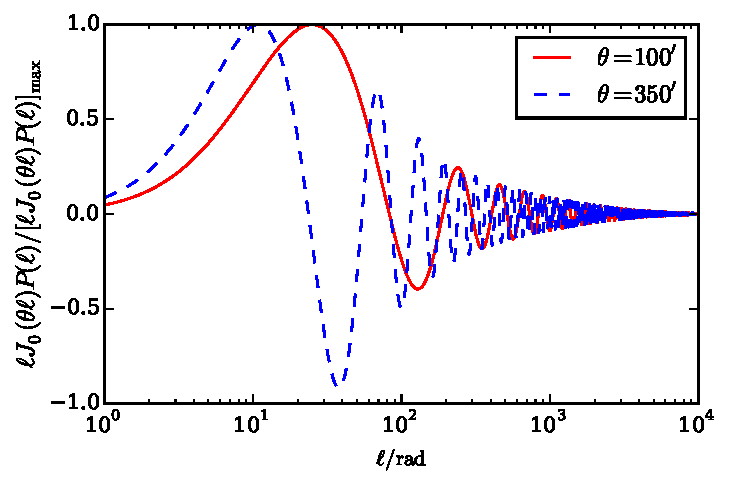
\includegraphics[width=0.325\textwidth]{figures/IntegKsip.pdf} 
%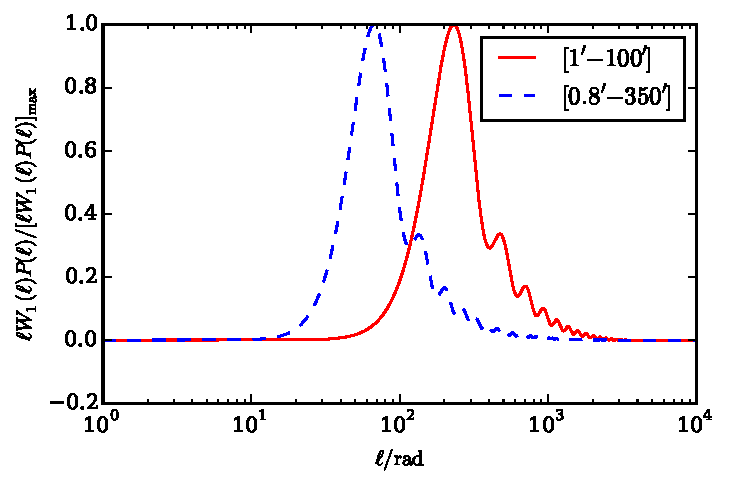
\includegraphics[width=0.325\textwidth]{figures/IntegCOSEBIs.pdf} 
%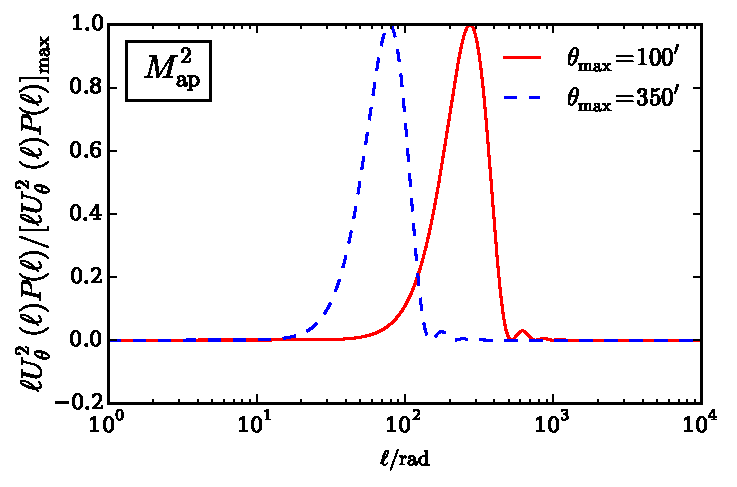
\includegraphics[width=0.325\textwidth]{figures/IntegMap.pdf}
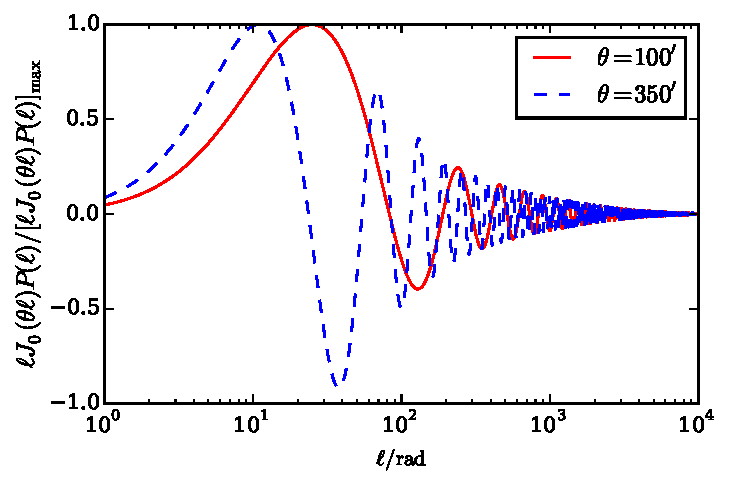
\includegraphics[width=0.65\textwidth]{figures/IntegKsip.pdf} \\
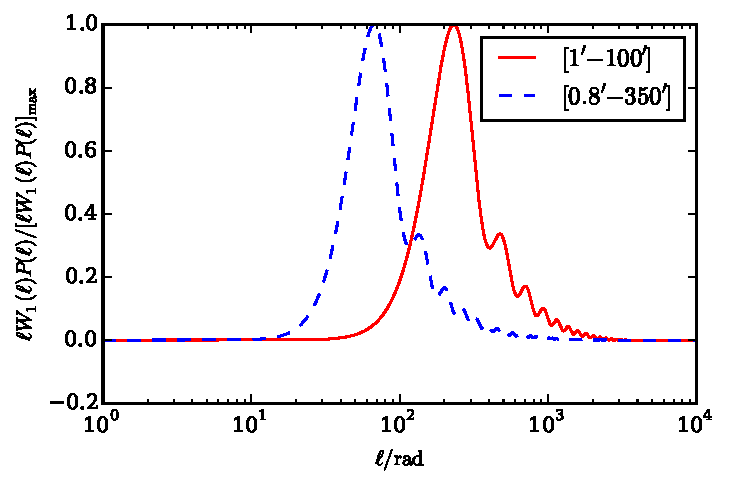
\includegraphics[width=0.65\textwidth]{figures/IntegCOSEBIs.pdf} \\
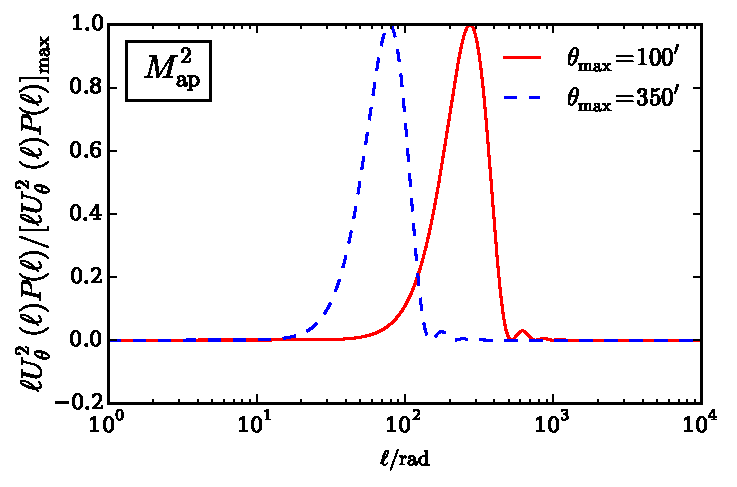
\includegraphics[width=0.65\textwidth]{figures/IntegMap.pdf}\\
\end{tabular}
\caption{ \small{\label{fig:filters}. Integrand of $\xi_+$ (upper), $E_1$ (middle, E-COSEBIs) and $\langle M_{\rm ap} \rangle^2$ (lower panel).
All integrands are of the form $\ell F(\ell) P(\ell)$, where $F(\ell)$ is the corresponding weight-function
for each statistic and $P(\ell)$ is the E-mode convergence power spectrum, with the exception of $\xi_+$, for which
$P(\ell)$ is equal to the sum of E and B-mode power spectra. 
Two cases are shown for each statistic as listed in each caption.
For the aperture mass statistic $\theta_{\rm max}=2\theta$ is shown. 
Note that higher order COSEBIs modes generally probe larger $\ell$-modes, 
hence here we only show the lowest mode $E_1$. All values are normalized with respect to their maximum value. }
}
\end{center}
\end{figure}

\subsection{On the Validation of Methods on Simulations}
It is discussed in \citet{kitching/etal:2016} that the validation of cosmic shear estimators on mock catalogues could also be affected by the approximations they investigate.  We agree that a full sky mock should be compared to a full curved sky non-Limber prediction.  It is then suggested, however, that the discrepancies already reported between existing mocks and the predictions could be attributed to these approximations, as opposed to a finite box effect \citep{kiessling/etal:2011, harnois-deraps/etal:2012, harnois-deraps/vanwaerbeke:2015}.  Going beyond flat-sky and Limber could improve the agreement, however this cannot explain the results of \citet{harnois-deraps/vanwaerbeke:2015} who demonstrate that the large-scale under-estimation of power varies with the simulation box size. This volume effect was verified by comparing explicitly the $\xi_+$ statistic at large angular scales between simulation volumes with box sides  ranging from 147$\rm{Mpc/h}$ to 515$\rm{Mpc/h}$ \citep[see Fig. 5 in][]{harnois-deraps/vanwaerbeke:2015}. The increase of power loss with decreasing box size was shown to be fully-modelled by excluding the super-box $k$-modes in the Limber predictions, something that the approximations discussed in \citet{kitching/etal:2016} would be unable to explain.

We note that any future comparison of mock data with full curved sky non-Limber predictions would place requirements on the input weak lensing simulations.  Many work with parallel plane mass-sheets as opposed to curved sky mass-sheets and at large angles these two approaches differ, regardless of the box size. 

\subsection{On the application to CMB lensing}
\citet{kitching/etal:2016} discuss how corrections to the Limber and flat-sky approximations would also affect predictions involving the shear and convergence cross-spectrum, such that the cross-correlation of CMB lensing and galaxy lensing should include a pre-factor $ [\ell(\ell+1)]^2/(\ell+ 0.5)^4$.   We have verified that this term would have negligible impact on current measurements, given the relatively low signal to noise ratio.  For example, most measurements \citep{hand/etal:2015, liu/hill:2015, kirk/etal:2016,harnois-deraps/etal:2016} are carried over angular multipoles in the range $\ell \in [20-2000]$.  The size of the pre-factor, averaged over this range, is of the order of 0.01\%. In comparison, the size of the statistical error bars are of the order 25-35\% with additional uncertainty due to photometric redshifts (10-15\%) and intrinsic galaxy alignments (10-15\%). The pre-factor reaches 1\% only for $\ell < 7$, which may become relevant for very large upcoming surveys but is negligible for current surveys. 

\subsection{On the quadratic estimator}

\citet{kitching/etal:2016} state that `the derivative of a Limber-approximated power spectrum is not equal to the Limber-approximation of the derivative'. Based on this statement they conclude that `statistics that use Limber-approximated quadratic estimators to measure the cosmic shear power spectrum are not accurate' and refer explicitly to the quadratic estimator implementation used in \citet{Koehlinger2016} to measure the cosmic shear power spectrum from CFHTLenS. In this quadratic estimator implementation, however, the Limber approximation does not enter. The algorithm was originally presented by \citet{Hu2001} in the context of cosmic shear and has also been applied to other shear data sets (e.g. \citealt{Brown2003, Heymans2005, Lin2012}). Below we briefly summarize this quadratic estimator algorithm and emphasize that the Limber approximation does not enter in there.

The aim of the method is to find the best-fitting power spectra assuming a Gaussian likelihood function $\mathcal{L}$. The likelihood depends on the shear data vector and its covariance $\mathbf{C}$ which consists of the sum of the shear correlation matrix $\mathbf{C}^\mathrm{sig}$ and the noise matrix $\mathbf{C}^\mathrm{noise}$. The shear correlation matrix can be written as a linear combination of piece-wise constant band powers $\mathcal{B}$ approximating the Fourier transforms of the shear correlations, i.e. their power spectra (cf. equations~3,~10 in \citealt{Koehlinger2016}). The best-fitting power spectra are found by iteratively stepping through a Newton--Raphson method in order to find the root of $\diff \mathcal{L}/ \diff \mathcal{B} = 0$ \citep{Bond1998, Seljak1998}. In the subsequent equations of the Newton--Raphson method only derivatives of the full covariance matrix enter, where the derivatives are taken with respect to band powers\footnote{i.e. $\partial \mathbf{C} / \partial \mathcal{B}_A$, where $A$ is a superindex over the type of the band, band-power bin and redshift correlation, see appendix\~A in \citealt{Koehlinger2016}.}.  The only approximation entering in the algorithm is the flat-sky approximation when introducing the Fourier decomposition of the spin-2 shear field.    This approximation is appropriate and accurate for current surveys as $\ell>80$  in all analyses published to date.
